%___________________________________________________________________
\begin{frame}[label=conclusion, standout]
  Fragen?
\end{frame}

\appendix

%___________________________________________________________________
\begin{frame}{Literatur}
  \nocite{*}
  \printbibliography[heading=none]
\end{frame}

%___________________________________________________________________
\begin{frame}[allowframebreaks]{Wichtige Konzepte im Training}


\textbf{Regularisierung:}
\begin{itemize}
    \item \textbf{Dropout:} Deaktiviert zufällig Neuronen während des Trainings, um Overfitting zu reduzieren und die Generalisierung zu verbessern.
    \item \textbf{Weight Decay:} Fügt einen Strafterm für große Gewichte hinzu und verhindert dadurch übermäßig komplexe Modelle.
\end{itemize}

\textbf{Feature-Reduktion:}
\begin{itemize}
    \item \textbf{MaxPooling:} Verringert die räumliche Auflösung von Feature-Maps, indem pro Bereich nur der größte Aktivierungswert beibehalten wird.  
    Reduziert Rechenaufwand und sorgt für Translationstoleranz (robuster gegenüber kleinen Verschiebungen im Bild).
\end{itemize}

\textbf{Optimierung:}
\begin{itemize}
    \item \textbf{Adam:} Optimierer, der Momentum und RMSProp kombiniert. Passt die Lernrate adaptiv für jedes Gewicht an.
    \item \textbf{Learning Rate:} Schrittweite, mit der die Gewichte in Richtung des Gradienten aktualisiert werden.  
    Zu groß → instabil, zu klein → langsames Lernen.
\end{itemize}

\end{frame}

% \improve{bessere farbpalette parallel_coordinate}
%___________________________________________________________________
\begin{frame}
  \begin{figure}
    \centering
    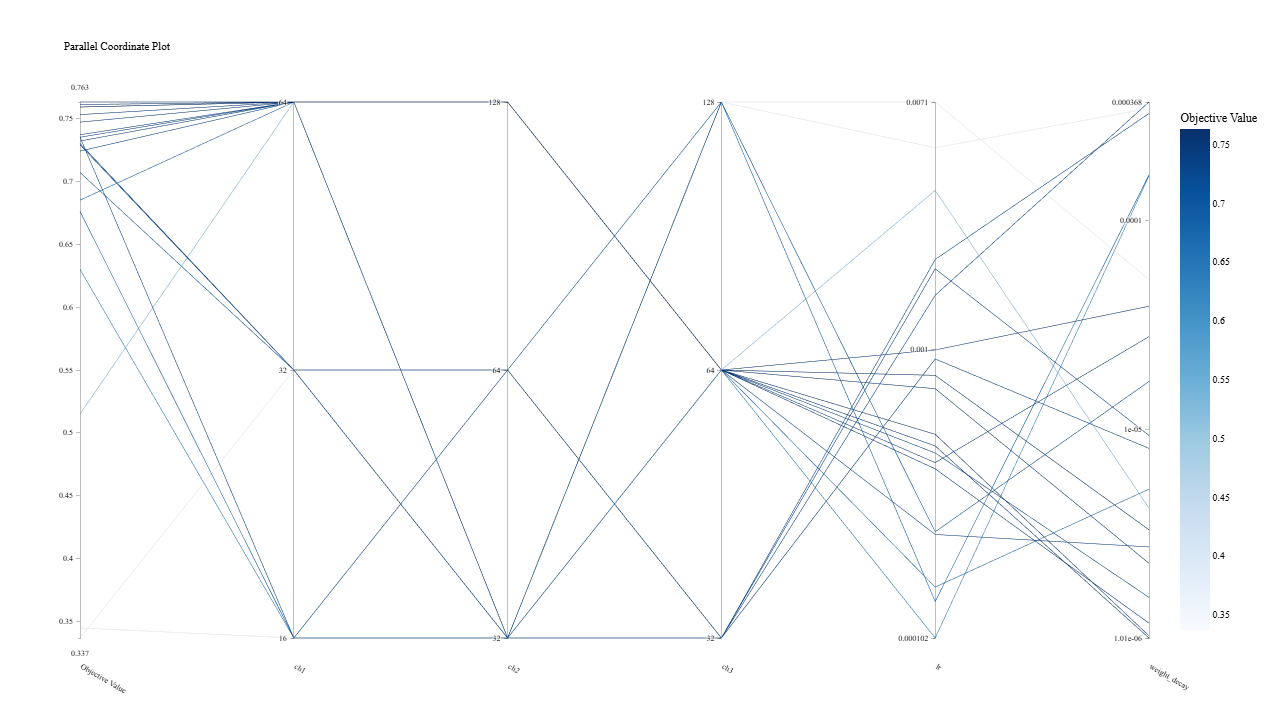
\includegraphics[width=\imagewidth, height=\imageheight, keepaspectratio]{parallel_coordinate.png}
  \end{figure}
\end{frame}

\begin{frame}
  \begin{figure}
    \centering
    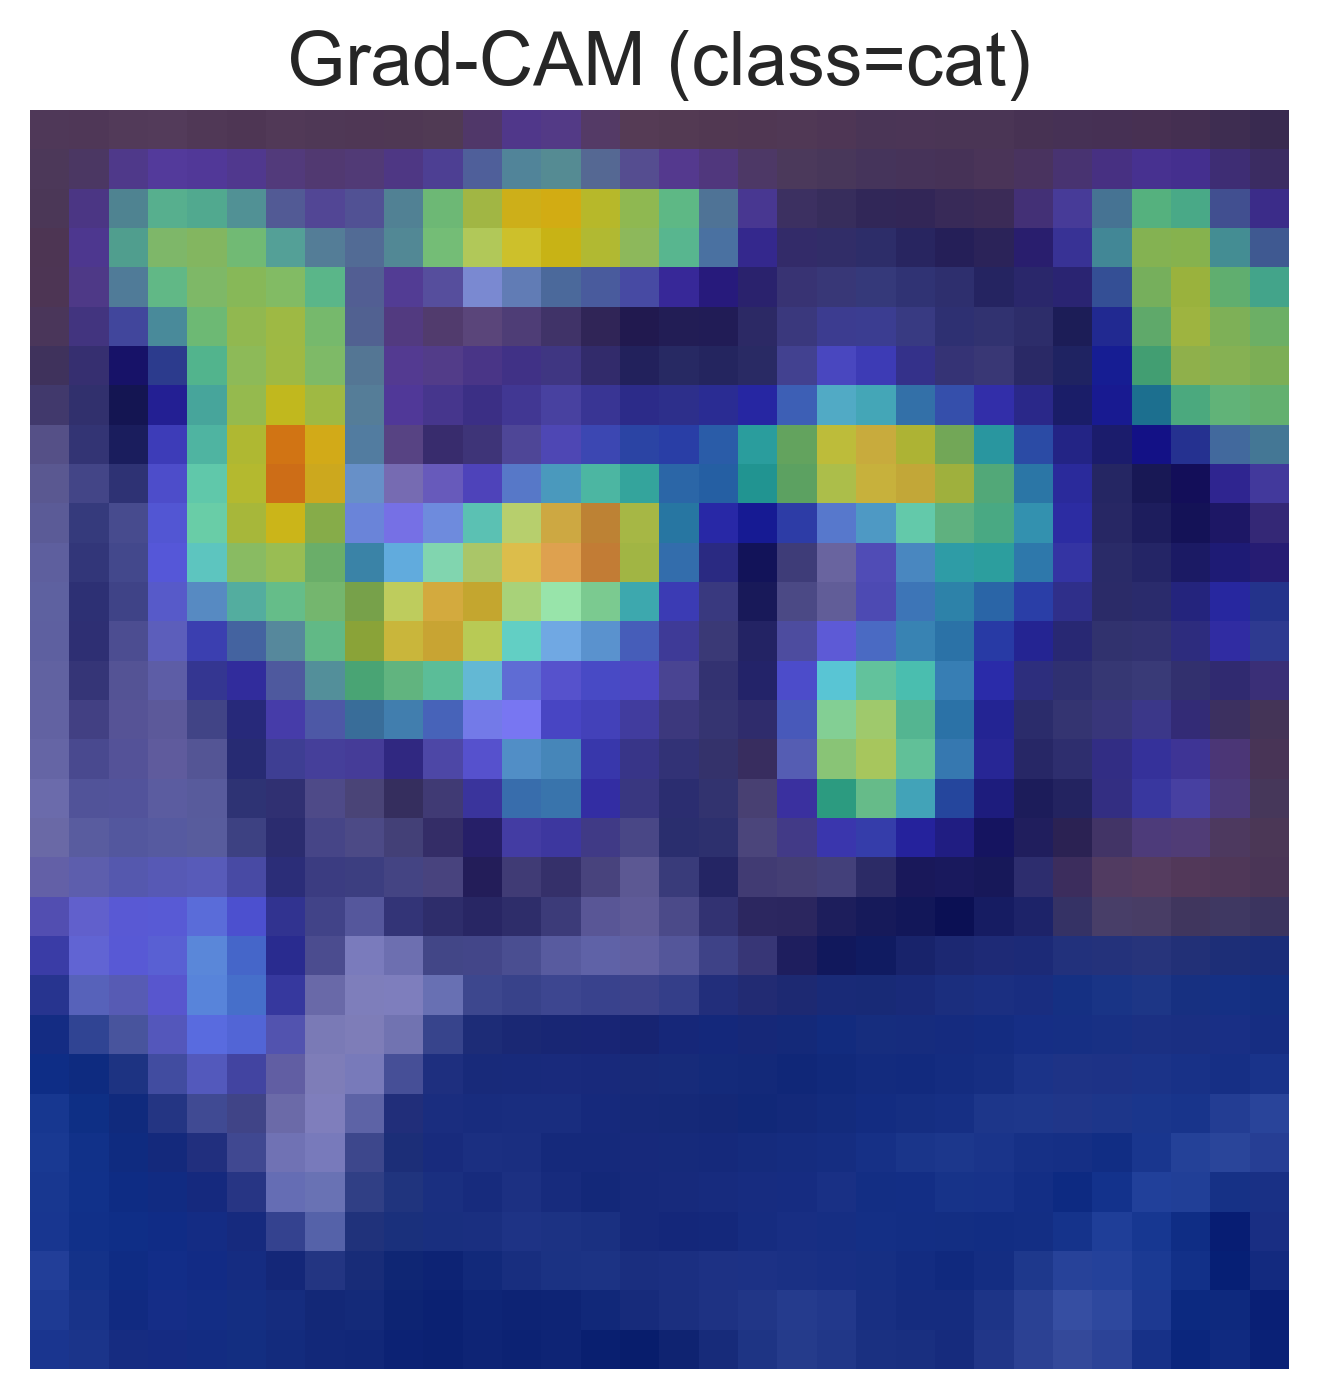
\includegraphics[width=\imagewidth, height=\imageheight, keepaspectratio]{gradcam.png}
  \end{figure}
\end{frame}

\begin{frame}
  \begin{figure}
    \centering
    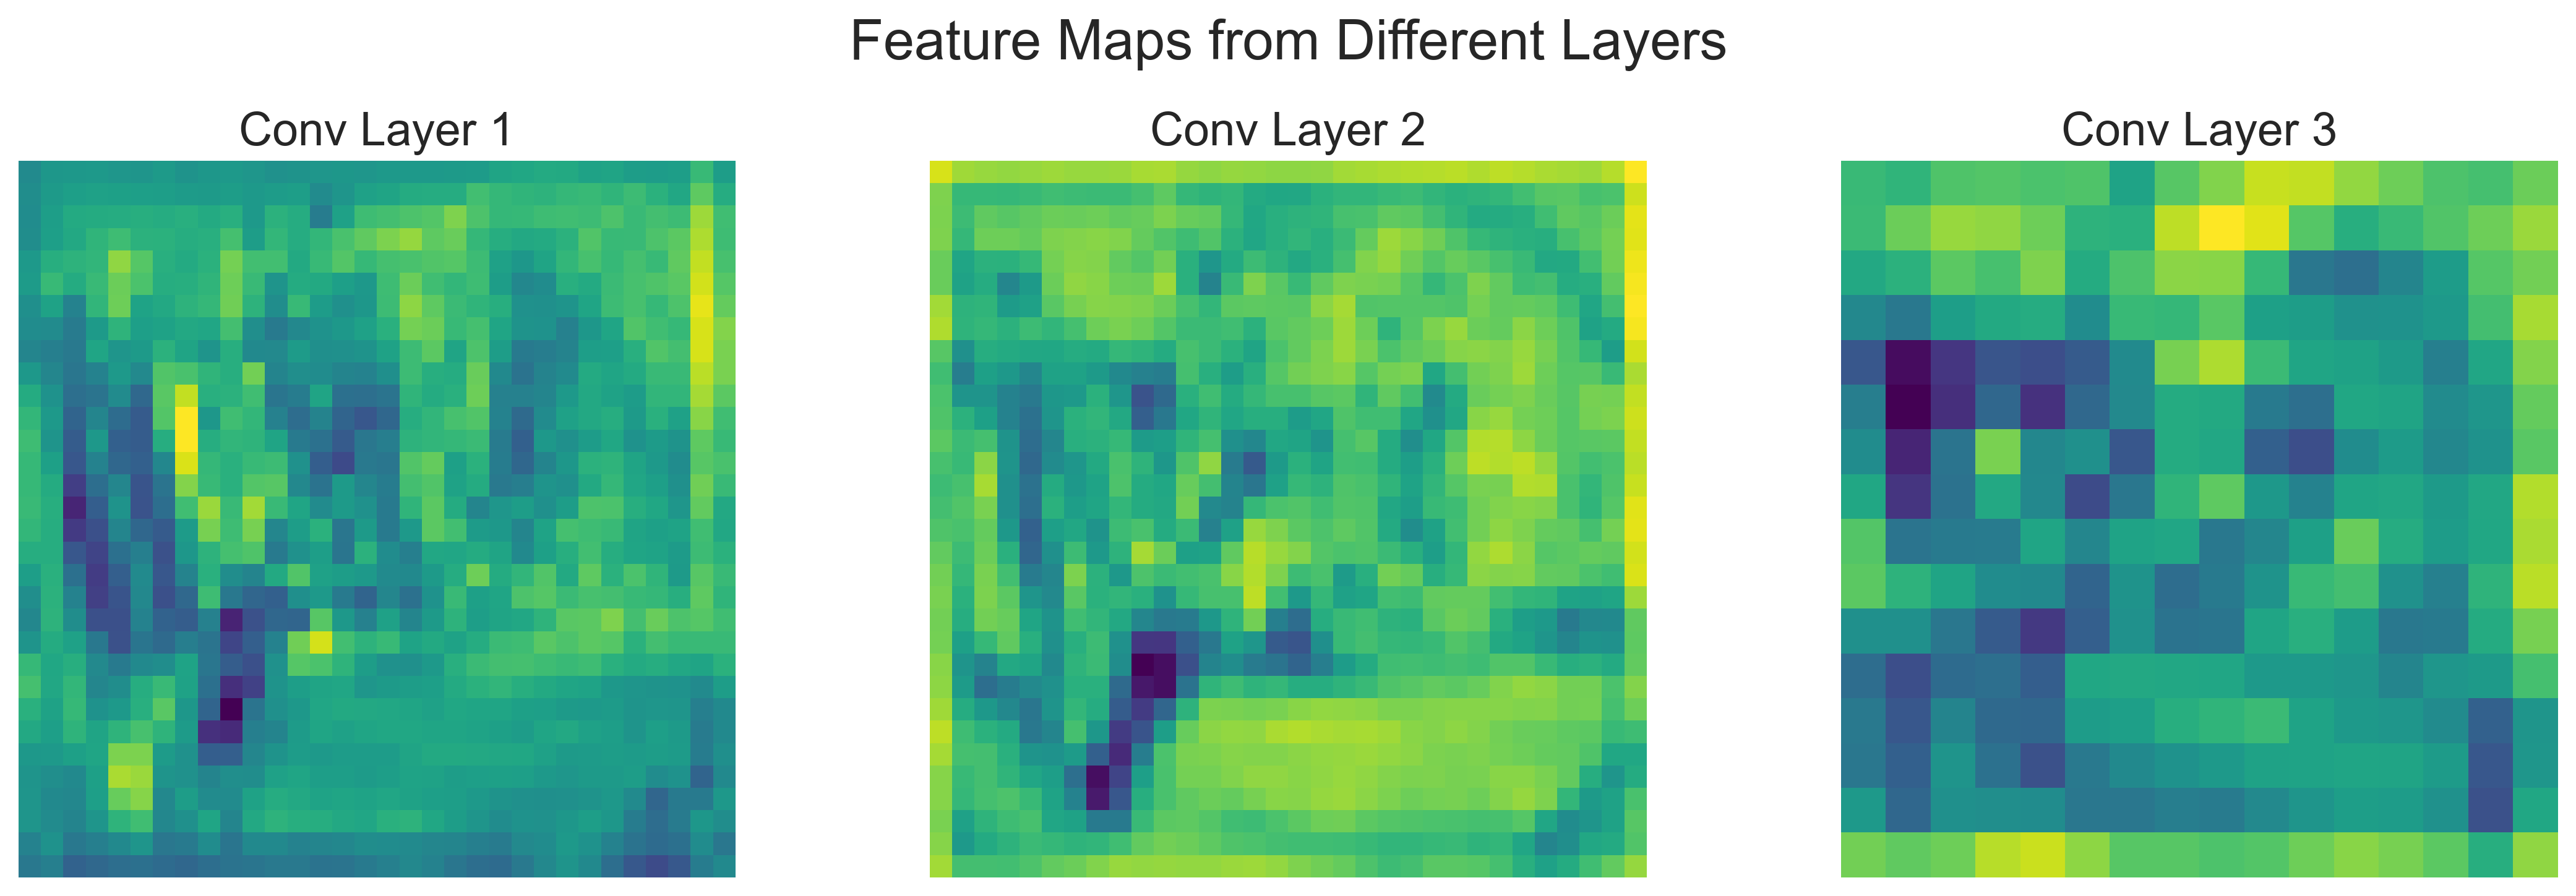
\includegraphics[width=\imagewidth, height=\imageheight, keepaspectratio]{feature_maps.png}
  \end{figure}
\end{frame}